\section{Introduction}
\label{sec:intro}

% Part 1: Text IE, scenarios, OCR
% What is text information extraction?
Information extraction is the task of automatically extracting information
or knowledge from unstructured or semi-structured documents.
In the domain of image processing,
the task of textual information extraction (TIE)
is automatically detecting and recognizing texts from given images.
% where is it used?
TIE is applied in a large variety of image categories,
such as printed books, newspapers, digital drawings,
or even more general images~\cite{jung2004text}.
% What's the kernel technique?
Optical character recognition (OCR) is the popular approach to solve TIE,
turning images of printed text into machine encoded texts.
OCR is a hot research topic in recent years, and the performance is promising
on \st{plain-text-based images} \KQ{images containing largely text},
such as novels and reports.
For example, Tesseract~\cite{smith2007overview},
one of the most popular open source multilingual recognizers,
achieved an error rate of 3.72\% for recognizing English words
and 3.77\% for simplified Chinese characters\cite{smith2009adapting}.
Based on the exclusive use and high accuracy of OCR,
the Google Books~\cite{vincent2007google} and Gutenberg Project~\cite{lebert2008project}
have scanned a large number of printed books
and converted into text for free and open access.

\begin{figure*}[!htb]
\centering
\subfloat[ECG]{
\label{fig:medicalimage:ecg}
\epsfig{file=figure/ECG.eps, width=1.10\columnwidth}
}
% % \hfill
% \subfloat[X-RAY]{
% \label{fig:medicalimage:xray}
% \epsfig{file=figure/X-RAY.eps, width=0.4\columnwidth}
% }
% \hfill
\subfloat[MRI]{
\label{fig:medicalimage:mrt}
\epsfig{file=figure/MRI.eps, width=0.88\columnwidth}
}
% \subfloat[EEG]{
% \label{fig:medicalimage:eeg}
% \epsfig{file=figure/EEG.eps, width=0.4\columnwidth}
% }
\caption{Examples of medical images with textual information.}
\label{fig:med-image-example}
\end{figure*}


% Part 2: Medical imaging, example image, raw OCR result (text + layout information)
% What's medical image, why important?
Due to ever evolving hardware and software, many medical images
such as electro-cardio graphs (ECGs), magnetic resonance imaging (MRI),
X-ray or ultrasound images are directly printed and stored
\st{in hard copy formats} \KQ{on paper}.
Medical images shown in \figref{fig:med-image-example}
contain a mix of graphics and text,
which include technical settings of the hardware used,
test measurements and simple diagnoses.
% TODO: why growing demand?
In order to build the manageable electronic medical records for patients,
there has been a growing demand for extracting such text-based
medical information from these medical images.
% What's the exmaple, and what's in the OCR output?
Given the ECG image in \figref{fig:running-ecg} as the running example,
existing OCR softwares are able to produce texts with spatial layout information,
indicating the positions of each recognized text in the image.
\figref{fig:running-xml} shows the raw OCR result produced by Tesseract,
where recognized texts are organized in the form of XML hierarchy of spans,
and we call them ``text boxes'' throughout this paper.
Texts are stored only in leaf text boxes,
and the layout information of each box is represented by
the coordinates (left, top, right, bottom) of its bounding box.
We use the term ``bounding box'' and ``zone'' interchangeably in this paper.
% TODO: Mention OCR error here??
It's worth mentioning that OCR softwares may generate incorrect texts.
for example, the original text ``Vent. rate'' in the image
is incorrectly recognized as ``Vcnt. rule'',
also ``63 bpm'' is recognized as ``53 bpm''.

\begin{figure*}[ht]
\centering
\epsfig{file=figure/running_ECG.eps, width=1.9\columnwidth}
\caption{An ECG with interesting text areas marked by red ovals.}
\label{fig:running-ecg}
\end{figure*}

% \begin{figure}[ht]
% \centering
% \subfigure[]{
% \label{fig:subfig:a}
% \begin{minipage}[b]{0.2\textwidth}
%\newsavebox{\firstlisting}
%\begin{lrbox}{\firstlisting}% Store first listing
%\begin{lstlisting}
%<p class='ocr_par' dir='ltr'>
%   <span class='ocr_line' id='line_2'>
%       <span class='ocrx_word' id='word_6'>Vent.</span>
%       <span class='ocrx_word' id='word_7'>rate</span>
%       <span class='ocrx_word' id='word_8'>65</span>
%       <span class='ocrx_word' id='word_9'>bpm</span>
%   </span>
%   <span class='ocr_line' id='line_3'>
%       <span class='ocrx_word' id='word_14'>PR</span>
%       <span class='ocrx_word' id='word_15'>interval</span>
%       <span class='ocrx_word' id='word_16'>162</span>
%       <span class='ocrx_word' id='word_17'>ms</span>
%   </span>
%    ...
%</p>
%\end{lstlisting}
%\end{lrbox}
% \end{minipage}
% }
% \hspace[1in]
% \subfigure[]{
% % \label{fig:subfig:b}
% % \begin{minipage}[b]{0.2\textwidth}
\newsavebox{\secondlisting}
\begin{lrbox}{\secondlisting}
% \tiny
\begin{lstlisting}[basicstyle=\tiny,]
<p class="ocr_par" title="box 263 33 444 119">
   <span class="ocr_l" title="box 264 33 336 45">
       <span class="ocrx_w" title="box 264 33 299 45">Vcnt.</span>
       <span class="ocrx_w" title="box 308 34 336 45">rule</span>
   </span>
   <span class='ocr_l'>
       <span class="ocrx_w" title="box 264 51 283 64">PR</span>
       <span class="ocrx_w" title="box 291 51 346 64">Interval</span>
       <span class="ocrx_w" title="box 389 52 411 64">140</span>
       <span class="ocrx_w" title="box 420 55 439 64">ms</span>
   </span>
   ...
   </span>
</p>
<p class="ocr_p" dir="ltr">
   <span class="ocr_l">
       <span class="ocrx_w" title="box 396 33 411 45">53</span>
       <span class="ocrx_w" title="box 420 33 449 48">bpm</span>
   </span>
</p>
\end{lstlisting}
\end{lrbox}
% % \end{minipage}
% }

% \KZ{\figref{fig:ocrre} is output from what software? Tesseract?}
\begin{figure*}[th]
%\subfloat[Image From Printer1]{
%\label{fig:ocrresub:a}
%\scalebox{0.8}{\usebox{\firstlisting}}}
%\hfill
%\subfloat[Image From Printer2]{
\scalebox{1.6}{\usebox{\secondlisting}}
% \label{fig:ocrre}
\caption{A fragment of raw OCR results for ECG with layout information.}
%\caption{Simplified OCR Results in XML for an ECG with Layout Information}
%\label{fig:ocrresub:b}
\label{fig:running-xml}
\end{figure*}

% \lipsum[2]



% Part 3: Goal of this paper: structured information (kv pair) extraction
%         Challenge: hard to write wrapper (professional, not friendly)
%                    noisy information & OCR error
%         direct approach: zonal approaches
%         weakness: error propagation
% kernel: structure --> pure OCR (text, regex based approach) is not reliable: not in a same box
% ZOI approach: zonal / page layout: inaccurate position (between diff. figures), error propagation

% What's the final goal?
Apart from scanning the images into digital formats,
extracting the structured textual knowledge is more important for
building electronic medical records.
% Using examples to illustrate.
For example in \figref{fig:running-ecg},
we would like to extract the attribute-value pairs
(e.g., \textit{Vent. rate = 63 bpm}) and possibly other values such as
date (e.g., \textit{18-Nov-2010}) and time (e.g., \textit{9:13:02}),
since those values endow us with information of the particular patient.
% Informally define the task
% Obviously, raw OCR results didn't explicitly encode such structured knowledge,
Since discovering structured knowledge is beyond the scope of the OCR techniques,
the goal of this work is to provide a systematic solution,
which enables users to easily specify the data of interest in the images,
and automatically extract the corresponding textual values from raw OCR results.

There are some naive solutions for this information extraction task.
% Naive approach 1: regex matching
The first approach is to write regex expressions for each data to be extracted,
and apply them to different text boxes of the OCR result.
For example, using \textit{``Vent\textbackslash . rate .* bpm''}
to capture the target bpm value.
However, this approach suffers from two major problems.
First and obviously,
incorrect recognized texts lead to mismatches of regex rules.
Second, the hierarchical layout of OCR results are
not always organized in a human-readable manner.
For example in \figref{fig:running-xml}, the text ``Vcnt. rule'' and ``53 bpm''
are not automatically combined into the same text box, but are rather far apart.
In fact, the hierarchical layout is sensitive to many factors,
including color, contrast, accidental spots on the prints, or the angle of the scanner camera.
In this case, text-based regex rules are not well suited for medical images.
Besides, writing regex rules is too ad-hoc and non-trivial for end users.

% Naive approach 2: ZOI based
The second approach is more straightforward:
the user first annotates all the target zones of each
\st{desired data} \KQ{piece of data},
then simply conducts OCR on each fragment of images.
Though intuitive and easy to implement,
this approach highly relies on the the accuracy of carefully annotated zones,
either too larger or too smaller will affect the local OCR results.
% TODO: why?? I don't know.
In addition, there exists slight positional variations of target zones
between two images, even if they share the same format.
Therefore, the user have to annotate zones for every individual image,
which is tedious and labour intensive.

% Naive approach 3: page layout
Another alternative solution involves the page layout analysis technique~\cite{o1993document},
which includes identifying and organizing the textual regions
in the scanned image of a text document.
\figref{fig:running-page-layout} shows the page layout result of the running example.
In particular, the technique first segments textual zones (blue blocks) from
non-textual zones and arrange them in their original order,
then detects individual text unit (red lines under texts) in each zone.
% Then in order to analyze the logical roles of the text zones
% (titles, captions, footnotes, etc.), logical layout analysis
% is used for labeling the semantics of the text zones.
Page layout analysis is mainly used for analyzing the semantics of text zones
for plain text image documents,
and it encounters two problems when applied to this task.
% When applied to structured TIE on medical images,
% this technique encounters two problems.
First, it is based on the strong assumption that images of the same format
share the same structure of page layout result.
Noises in the image will affect the page layout result and
eventually generate totally error textual information.
Second, users must implement an addition wrapper to describe the location
(which texts in which regions) of each desired data.
This step highly depends on the detail result of page layout,
and writing such wrapper is almost intractable
for common users without expert knowledge.
% The page layout analysis technique is used to determine where the text
% resides on a page ,
% % By using page layout analysis technique, the hierarchy of physical components
% % can be generated and to match with the hierarchy of logical components, which
% % is predefined.
% The problem with applying
% such technique on medical images is that it creates so much noises
% that performance is ultimately affected.
% For medical images like ECG, useful information is often
% found in the small components of the image, while most of the images are
% regarded as noises.
% % check paper and more description, weakness, ref
\begin{figure*}[ht]
\centering
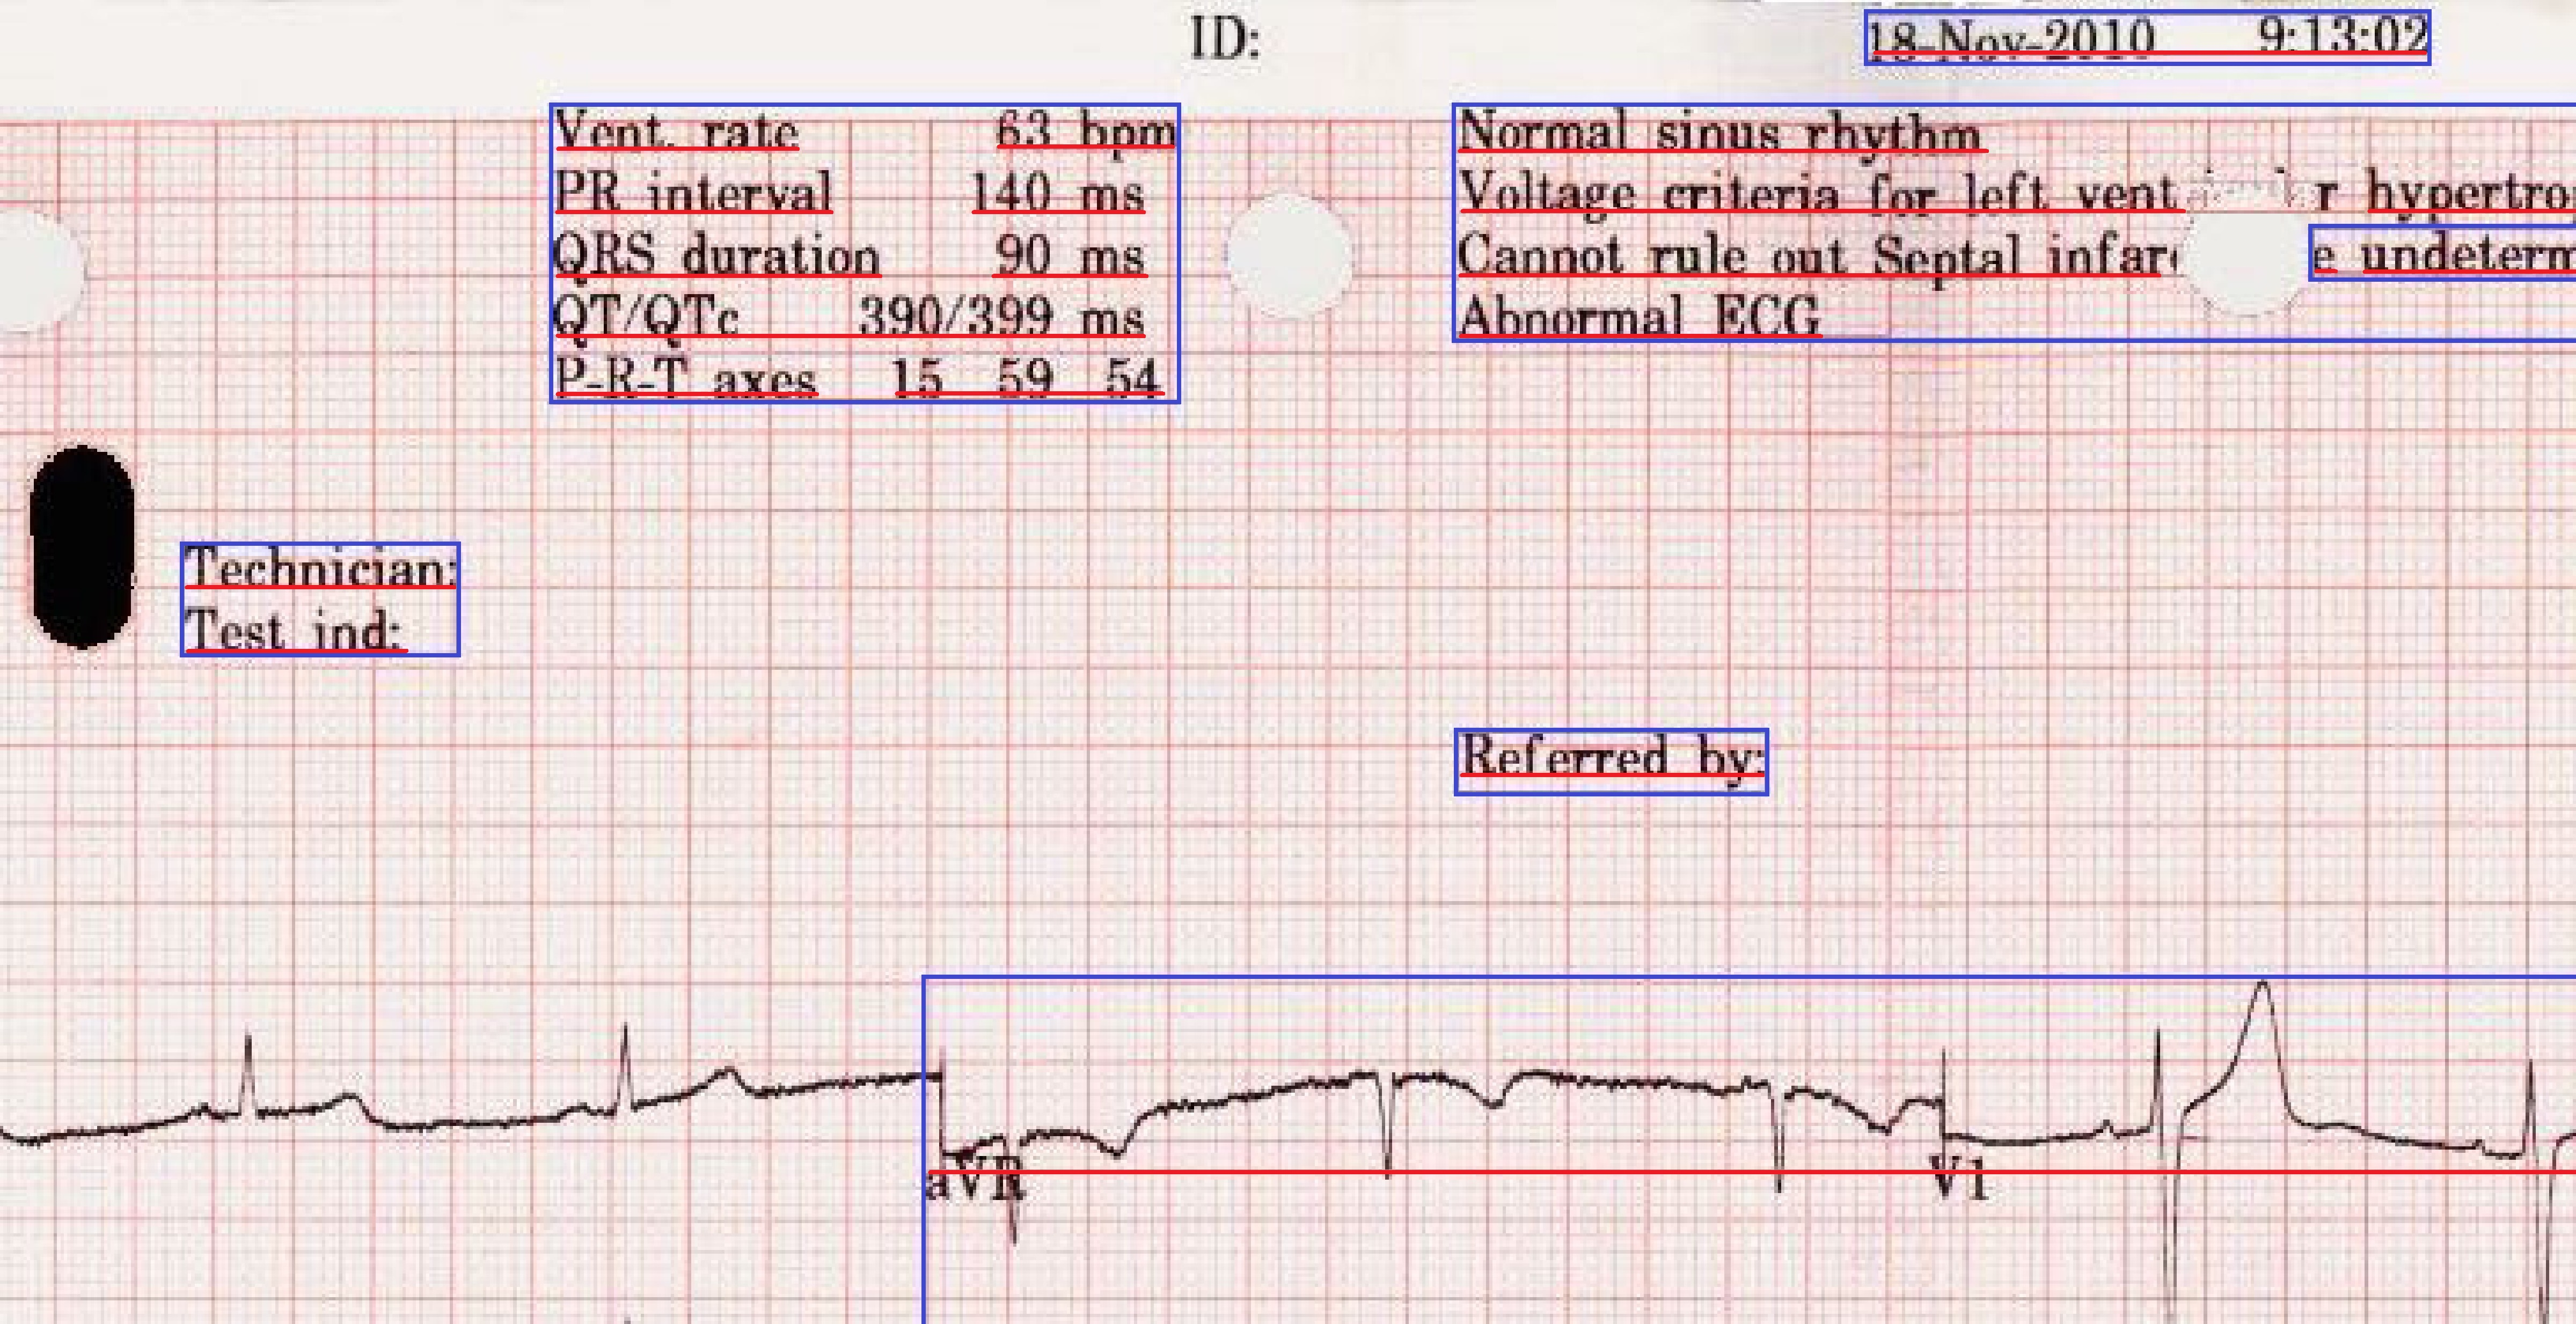
\epsfig{file=figure/page_layout.jpg, width=1.9\columnwidth}
\caption{Example result of page layout analysis.}
\label{fig:running-page-layout}
\end{figure*}

% Part 4: Our approach: ODL based (in fact we are writing a parser)
%         user-friendly;
%         present spatial information via element order (LR, UD) and rough spatial constraints, without too precise position
%         What's more: support error prompt and automatic correction based on OCR info & human correction.
% to solve: treat as an alignment problem: find the best alignment between var and box,
%       satisfying both data-level and spatial-level constraints.
% Challenge: How to measure the spatial-level fitness without hard code position information?
% Our approach: DSL-based, 3 advantages:
%    1. user-friendly: simple syntax to describe what's in the image, and what's the data-of-interest. all need: following left-to-right and top-to-bottom style.
%    2. robust and efficient alignment (fuzzy): leverage relative position and rough coordinates defined in ODL tolerant position delta
%    3. correction model: automatic made correction based on OCR and human feedbacks, and prompt errors to easily tell user what's wrong.

% 1. avoid what, our intuition is?
In order to attack the limitations of the above approaches,
We propose a domain-specific language for describing and extracting
structured textual information from the raw OCR data of medical images.
We call it OCR description language, or ODL in short.
The ODL parser then parses the raw OCR data
of the medical images according to the description,
and extracts structured textual data in a tree shape.
The ODL based solution has three major advantages.
% adv 1. user-friendly
First, compared with the previous methods, ODL is more user-friendly.
%Instead of writing ad-hoc wrappers,
Borrowing the syntax from PADS~\cite{fisher2005pads},
an ad-hoc data processing language,
ODL provides a concrete syntax which allows users to easily define
fixed strings and variables to be extracted,
customize compositions for better organizing structured data,
apply value constraints on variables, and rough spatial constraints on structures.
% adv 2. layout-aware
Second, the syntax of ODL is layout-aware.
Besides the explicit description of the bounding boxes of individual data,
ODL also implies the relative layout between different data elements,
which is based on the left-to-right and top-to-bottom data description manner.
Those rich layout information support the effectiveness of the ODL parser.
% so that ODL implies the relative layout between different elements.
% adv 3. robust and efficient alignment
Third, the parsing process of ODL is robust.
Intuitively, the process aims at finding the best alignments
between the data defined in ODL and the text boxes of the raw OCR result,
satisfying both value constraints,
spatial constraints and their relative layouts.
The fuzzy matching strategy is applied to tolerate
or even automatically correct recognition errors brought by OCR,
as well as slight layout variances between images.
Therefore, neither carefully annotated zones nor
perfect OCR recognitions are required in the extraction step.
% % adv 3. automatic correction
% Third, the extraction results of ODL can be further
% improved by automatic correction.
% ODL is able to detect imperfect alignments via
% string mismatches or constraint violations,
% and then prompts the user to manually correct prominent parsing errors.
% These manual corrections serve as incremental annotations,
% which update the fuzzy matching strategy, and produce better extraction results.

% Or: 1. user friendly; 2. rich spatial semantics (implicit, explicit); 3. fuzzy


% Part 5: In summary, bullets.
In summary, this paper makes three main contributions.
\begin{enumerate}
\item We design a declarative spatial data description language
for describing both spatial and value constraints in medical images,
which can be used to automatically generate parsers for
structured information extraction from these images.
The syntax of ODL can be generalized to
%textual information extraction on
the other image domains (\secref{sec:syntax});
\item We propose a robust ODL parser,
which builds the association between the text boxes from raw OCR results
and the corresponding description in ODL.
During the parsing phase, the parser is able to tolerate
the noises and errors brought by OCR recognition,
as well as inaccurate bounding boxes of input description (\secref{sec:parsing});
\item We conduct preliminary experimental studies of
structured information extraction on real ECG dataset.
The end-to-end evaluation result shows that our ODL based solution
consistently outperforms existing approaches.
Besides, the extraction accuracy further increases by 2\%,
given only a few number of manual corrections.
(\secref{sec:eval}).
\end{enumerate}
